\section{Speed layer}
\label{sec:speed_layer}

To overcome delay of the batch processing the Lambda architecture has the speed layer.
It applies the real-time incremental processing to arriving data.
The speed layer has higher complexity than the batch layer, because of the incremental nature of applied algorithms.
It provides usually approximated results, because algorithms, used for online processing, are often approximated.

The speed layer computes real-time views, that are similar to batch views in the sense, that they store data useful for fast answering queries.
Real-time views contain data, observed during ongoing batch processing in the batch layer.
The speed layer also prepares indexes on those views, that allow to answer queries ``on the fly''.
The general structure of the Speed layer is present on the Fugire~\ref{fig:SpeedLayer}.

\begin{figure}[h]
  \centering
  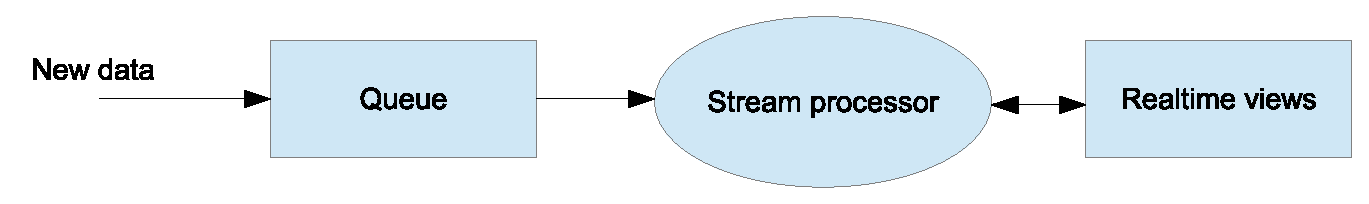
\includegraphics [width=1.0\textwidth]{images/SpeedLayer}
  \caption{The general structure of the Speed layer.}
  \label{fig:SpeedLayer}
\end{figure}

\subsection{Computation of real-time views}

To compute real-time views, one could consider the same approach as for batch views, but use only new data for computations.
This would simulate batch processing on the much smaller scale.
Nevertheless, if we want to achieve latency of miliseconds, such approach is not going to work.
Batch processing even on the scale of several gigabytes is not possible to do in miliseconds.

To solve this issue there is a completely different approach.
Real-time views are not considered as a function of a recent data, that has arrived during current batch processing.
Instead, they are the result of the function of a new data, that just came, and of their previous state.
Basically, it is an incremental update with a small piece of data, everytime it arrives.
This normally leads to only approximated answers to the queries, provided by real-time views.
But this is again not a problem, because error does not accumulate for too long.

\subsection{Data storage}

Speed layer must obey low-latency requirement, and must allow application complex incemental algorithms.
Having such demands, storing of real-time views requires several properties to be fulfiled: ability to make random reads and writes, scalability and fault-tolerance.
Ability to make random reads is particularly important to make answering queries fast.
Ability to make random writes is necessary, because of the need to apply incremental algorithms, that always demand this property.
Real-time views must be scalable, because amount of data to process can still be of a huge size.
That means, that distribtuion to many machines must be supported.
Fault-tolerance is as usual must be provided via replications of data in the real-time views.

There are many storage systems, that fulfil these properties.
They are usually called \textit{NoSQL databases}\mnote{NoSQL database}.
They store data using different data models than relational databases.
We have already briefly discussed one of such system, namely ElephantDB, that was useful for storing batch views in the serving layer.
One can choose specific database, that fulfils his or her requirements to data representation.
Sometimes batch and real-time views has the same data format.
But it is not always the case, because it is not always easy to execute the same function in the batch and in the incremental way.
Also, as long as real-time views have to be updated incrementally, they have more complex data structure.
Because of those factors, it often happens, that real-time views represent data differently, than batch views.

\subsection{Issues of incremental computations}

We have already discussed the difference between incremental and recomputation algorithms.
Batch computations imply, that computations of a specific function is executed on the whole dataset.
This is usually easy to program, even though can take much time.
In case of incremental computations, building of real-time view is going continuously.
It is usually more efficient, but can lead to accumulation of error, especially if programming mistake takes place.

The important aspect to discuss it a relation of incremental computations and a so called CAP theorem.
The CAP theorem states, that consistency and availability are not possible simultanously to achieve, when data is partitioned.
The meaning of the CAP theorem is that it is possible to make the system completely available, but it can sometimes return not yet actual data, or it is possible to make it truly consistent, but it can sometimes provide now response for a request, because data is not yet propogated to partitions.

There several ways of how to design the system, so that it provides consistency or availability completely, or has a tradeoff between them.
System is fully consistent, if it updates all replicas of a piece of data at once, and only then allow to access this data.
It is fully available, if it stores an update as a new temporal record, and then tries to merge it with the real data in the system.
This can take time, and reading of that data can return old values.

To achieve a tradeoff there so called \textit{conflict-free replicated datatypes} (CRDTs).
They provide eventual consistency working in a distributed fashion.
For example the G-Counter allows to maintain a counter, that allows only incrementation.
It stores different versions of an integer counters in different replicas, and the merge them to provide correct results.
There is unfortunately no way to aboid this complexity, and to make the system fully consistent and available at once.

\subsection{Expiration period of real-time views}

Real-time views, though more complex than batch views, but have only transient nature.
They are discarded every time, when batch layer completes processing of batch views.
Batch views then contain all information, that real-time views gathered during the last batch processing. 
Such temporal nature of real-time views saves from accumulation of error, and leads to eventual accuracy of query answering.

The simplest solution of discarding old real-time views is to set expiration time or period.
But it suffers from unstability of the duration of batch processing, that can vary every time.
Because of that, more robust, generic solution were proposed.

Let us consider a new information system, that does not have yet any data.
On the first run of batch processing the master dataset is empty.
But it still takes time, let say 10 minutes, because of overhead for creation of empty views, indexes, and so forth.
The speed layer gathers during this first batch processing data, and to its end has already real-time views, containing data, processed during this 10 minutes.

When the second start of batch computations runs, it consider the first 10 minutes of data, that resides now in the master dataset, for processing.
The speed layer continues to update real-time views.
Let's say the second batch processing takes 15 minutes.
To its end batch views have the reflection of the first 10 minutes.
Real-time views reflect all 25 minutes of system's life.
Now the part of them, that was built during th first 10 minutes can be discarded.

When the third batch processing starts, it considers data gathered during 25 minutes.
The online processing in the speed layer has updates now views, that has 15 minutes of processed data, gathered during the second batch processing.
Let's say the batch processing takes 18 minutes now.
When it finishes, batch views reflect the first 25 minutes of data, whereas real-time views reflect 33 minutes of data, starting after 10 minutes of the system's functioning.
Now real-time views must leave only reflection of the last 18 minutes of arriving data.

To make it possible, two sets of real-time views must be maintained.
The speed layer then switch between them after each finish of the batch processing.
Each set of real-time views store them results of processing during two consecutive batch runs.
This can look redundant and expensive, but is actually not, because real-time views store only small data, gathered during short time.
